\section{Extended Results and Error Analysis}\label{sec:extended}
\subsection{Complete control intervals}
\Figref{fig:controls} shows marginal 95\% prompt-bootstrap intervals for instruction controls. \Tabref{tab:extendedstyle} and \tabref{tab:extendedquality} list all individual conditions, including each random direction and the base signed doses, directly from the cached paired-comparison table. Style tests outside the two primary instruction mean $-2$ contrasts are exploratory; the plotted intervals are not simultaneous across conditions.
\begin{figure}[ht]\centering
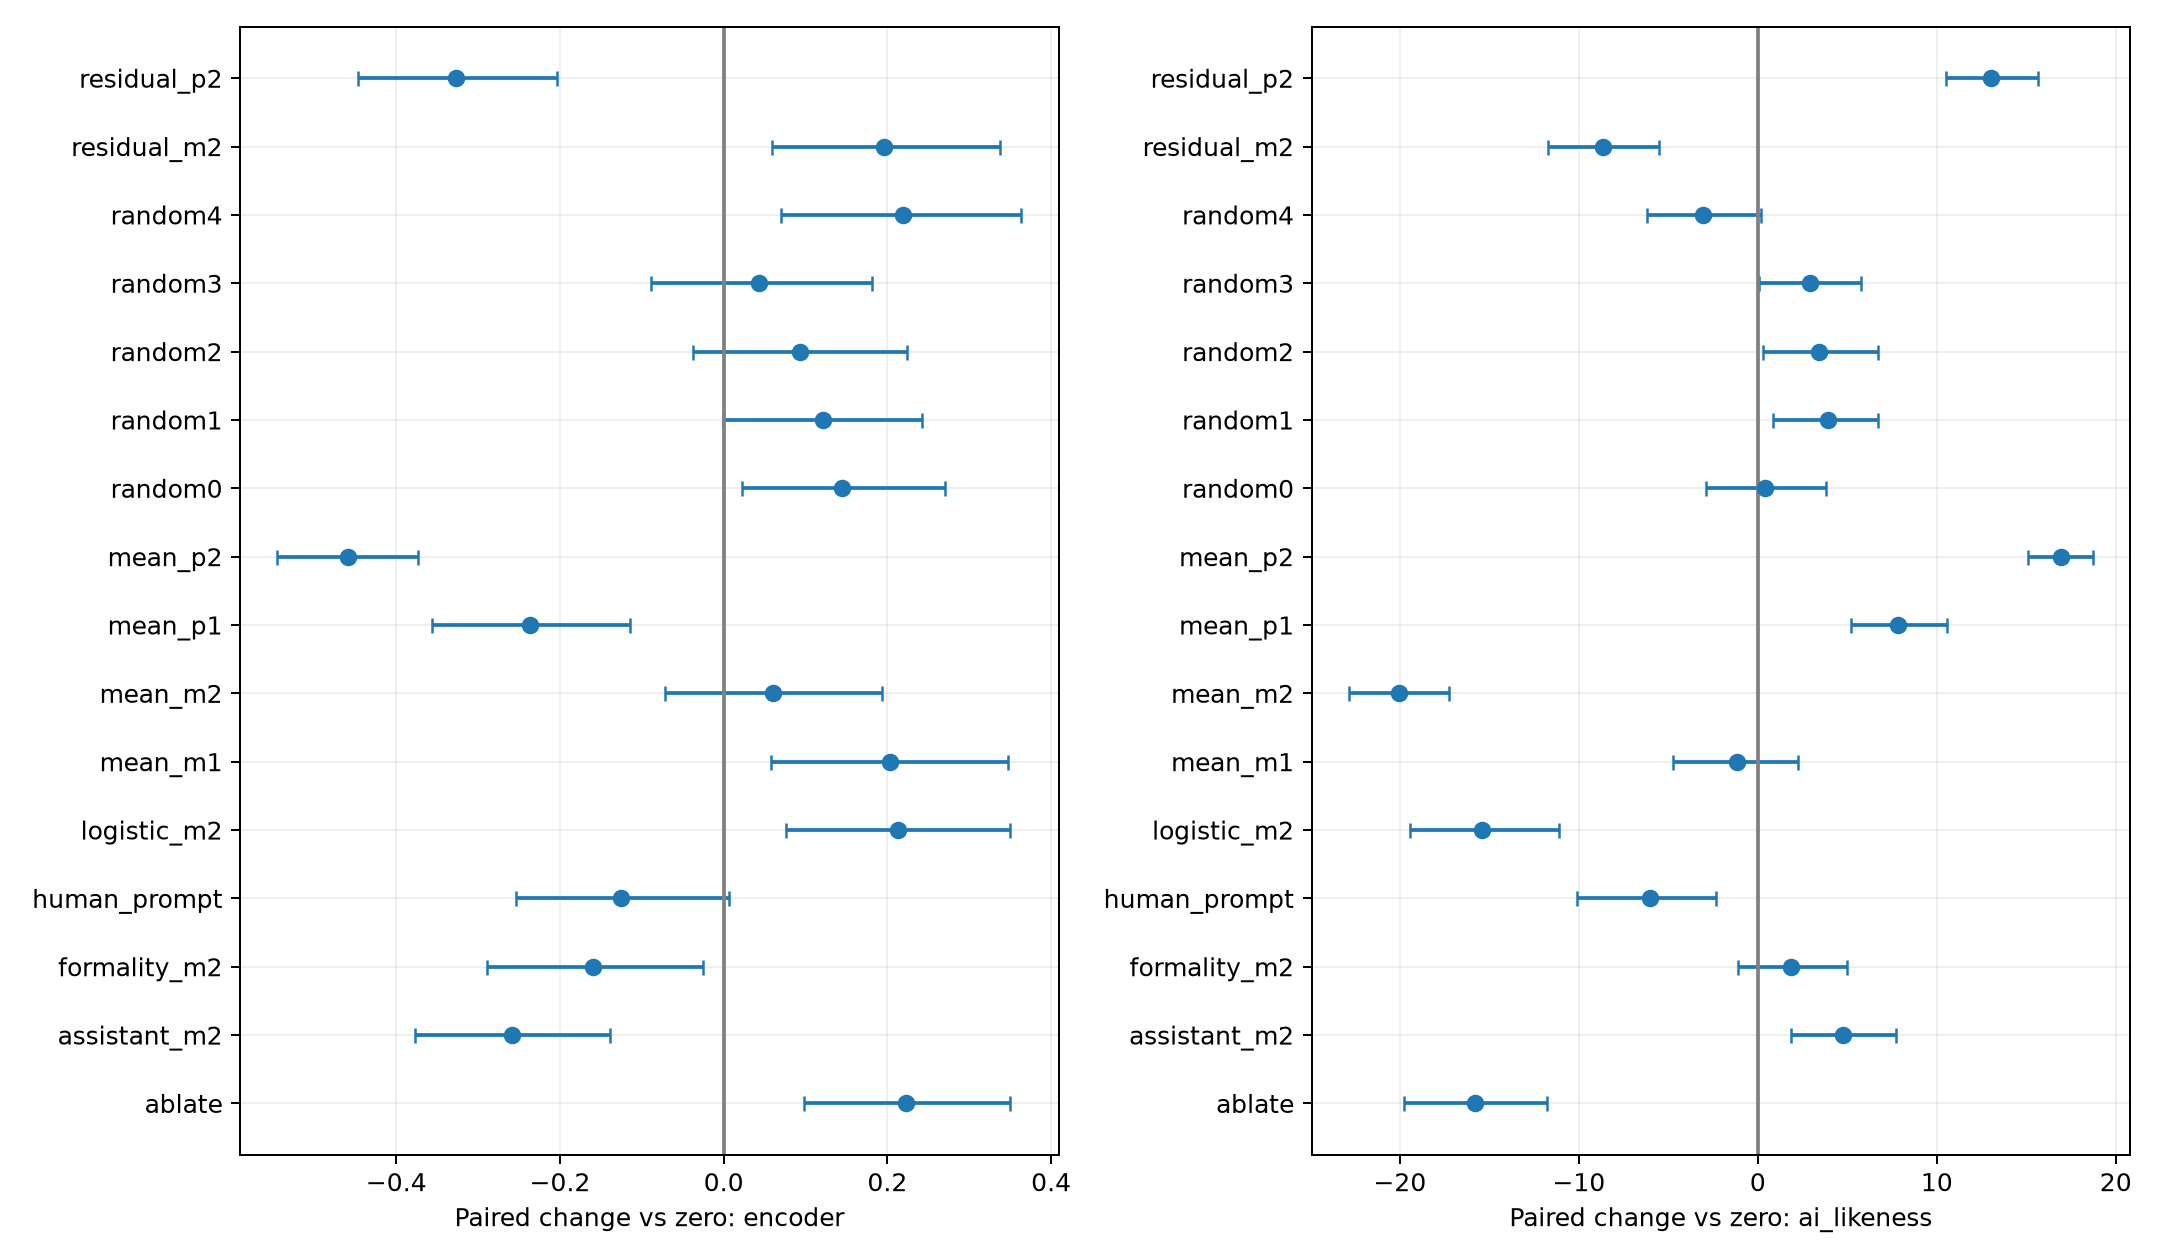
\includegraphics[width=0.95\linewidth]{figures/controls.png}
\caption{Instruction-model control contrasts relative to paired zero outputs. Points and bars show mean changes and marginal prompt-bootstrap 95\% CIs. Mean $\pm2$ uses two seeds per prompt; other conditions use seed 42. The large negative judged effect of mean $-2$ accompanies coherence loss and is not corroborated by the encoder.}\label{fig:controls}
\end{figure}
\begin{table}[htbp]\centering\scriptsize
\caption{All paired style changes [95\% CI], 64 records per row. Instruction mean $\pm2$ uses two seeds; other rows use seed 42. Comparisons use matching zero seeds.}\label{tab:extendedstyle}
\resizebox{\textwidth}{!}{\begin{tabular}{@{}llll@{}}
\toprule
Backbone & Condition & Judge AI-likeness & Encoder probability\\\midrule
Instruction & Ablation & $-15.781\;[-19.766,-11.797]$ & $+0.223\;[+0.098,+0.350]$\\
Instruction & Assistant $-2$ & $+4.766\;[+1.873,+7.734]$ & $-0.259\;[-0.377,-0.138]$\\
Instruction & Formality $-2$ & $+1.875\;[-1.094,+5.000]$ & $-0.159\;[-0.289,-0.025]$\\
Instruction & Human prompt & $-6.016\;[-10.078,-2.344]$ & $-0.126\;[-0.254,+0.007]$\\
Instruction & Logistic $-2$ & $-15.391\;[-19.453,-11.094]$ & $+0.214\;[+0.076,+0.350]$\\
Instruction & Mean $-1$ & $-1.172\;[-4.766,+2.266]$ & $+0.203\;[+0.058,+0.347]$\\
Instruction & Mean $-2$ & $-20.039\;[-22.852,-17.266]$ & $+0.061\;[-0.072,+0.193]$\\
Instruction & Mean $+1$ & $+7.844\;[+5.188,+10.548]$ & $-0.237\;[-0.356,-0.114]$\\
Instruction & Mean $+2$ & $+16.930\;[+15.102,+18.719]$ & $-0.459\;[-0.545,-0.373]$\\
Instruction & Random 1 & $+0.391\;[-2.891,+3.828]$ & $+0.144\;[+0.023,+0.271]$\\
Instruction & Random 2 & $+3.906\;[+0.859,+6.719]$ & $+0.121\;[-0.001,+0.242]$\\
Instruction & Random 3 & $+3.438\;[+0.312,+6.719]$ & $+0.093\;[-0.038,+0.224]$\\
Instruction & Random 4 & $+2.891\;[+0.078,+5.781]$ & $+0.043\;[-0.089,+0.181]$\\
Instruction & Random 5 & $-3.047\;[-6.172,+0.156]$ & $+0.219\;[+0.070,+0.364]$\\
Instruction & Residualized $-2$ & $-8.672\;[-11.719,-5.547]$ & $+0.196\;[+0.059,+0.338]$\\
Instruction & Residualized $+2$ & $+13.000\;[+10.500,+15.656]$ & $-0.327\;[-0.447,-0.204]$\\
Base & Mean $-2$ & $-12.812\;[-18.281,-7.031]$ & $-0.244\;[-0.365,-0.124]$\\
Base & Mean $+2$ & $+38.344\;[+32.516,+44.062]$ & $-0.429\;[-0.543,-0.315]$\\
\bottomrule
\end{tabular}}
\end{table}

\begin{table}[htbp]\centering\scriptsize
\caption{All paired quality changes [95\% CI], 64 records per row. Instruction mean $\pm2$ uses two seeds; other rows use seed 42. Comparisons use matching zero seeds.}\label{tab:extendedquality}
\resizebox{\textwidth}{!}{\begin{tabular}{@{}lllll@{}}
\toprule
Backbone & Condition & Coherence & Coverage & Unsupported\\\midrule
Instruction & Ablation & $-0.233\;[-0.453,-0.006]$ & $-0.002\;[-0.039,+0.035]$ & $-0.023\;[-0.059,+0.012]$\\
Instruction & Assistant $-2$ & $+0.125\;[-0.062,+0.312]$ & $-0.051\;[-0.097,-0.005]$ & $-0.012\;[-0.044,+0.020]$\\
Instruction & Formality $-2$ & $+0.062\;[-0.109,+0.250]$ & $-0.071\;[-0.110,-0.030]$ & $-0.013\;[-0.041,+0.016]$\\
Instruction & Human prompt & $-0.094\;[-0.328,+0.141]$ & $-0.024\;[-0.061,+0.011]$ & $+0.001\;[-0.029,+0.030]$\\
Instruction & Logistic $-2$ & $-0.570\;[-0.844,-0.297]$ & $-0.039\;[-0.077,-0.002]$ & $+0.023\;[-0.012,+0.058]$\\
Instruction & Mean $-1$ & $-0.234\;[-0.469,+0.000]$ & $-0.012\;[-0.054,+0.028]$ & $-0.011\;[-0.042,+0.022]$\\
Instruction & Mean $-2$ & $-0.591\;[-0.754,-0.427]$ & $-0.028\;[-0.057,+0.002]$ & $+0.014\;[-0.014,+0.042]$\\
Instruction & Mean $+1$ & $+0.052\;[-0.141,+0.250]$ & $-0.043\;[-0.084,-0.005]$ & $+0.019\;[-0.017,+0.054]$\\
Instruction & Mean $+2$ & $-0.414\;[-0.551,-0.281]$ & $-0.131\;[-0.164,-0.100]$ & $+0.093\;[+0.072,+0.114]$\\
Instruction & Random 1 & $-0.109\;[-0.328,+0.086]$ & $-0.016\;[-0.053,+0.021]$ & $+0.024\;[-0.011,+0.059]$\\
Instruction & Random 2 & $+0.000\;[-0.188,+0.203]$ & $-0.005\;[-0.042,+0.033]$ & $+0.035\;[-0.002,+0.073]$\\
Instruction & Random 3 & $+0.148\;[-0.047,+0.344]$ & $+0.016\;[-0.020,+0.052]$ & $-0.009\;[-0.038,+0.021]$\\
Instruction & Random 4 & $-0.164\;[-0.383,+0.062]$ & $-0.025\;[-0.067,+0.017]$ & $+0.043\;[+0.005,+0.081]$\\
Instruction & Random 5 & $-0.120\;[-0.345,+0.102]$ & $-0.006\;[-0.047,+0.035]$ & $-0.019\;[-0.053,+0.015]$\\
Instruction & Residualized $-2$ & $-0.555\;[-0.766,-0.344]$ & $-0.045\;[-0.087,-0.006]$ & $-0.003\;[-0.037,+0.030]$\\
Instruction & Residualized $+2$ & $-0.406\;[-0.641,-0.172]$ & $-0.111\;[-0.160,-0.061]$ & $+0.064\;[+0.030,+0.098]$\\
Base & Mean $-2$ & $-0.094\;[-0.320,+0.133]$ & $+0.002\;[-0.034,+0.038]$ & $-0.018\;[-0.049,+0.010]$\\
Base & Mean $+2$ & $-0.292\;[-0.534,-0.042]$ & $-0.215\;[-0.267,-0.161]$ & $+0.189\;[+0.144,+0.231]$\\
\bottomrule
\end{tabular}}
\end{table}

\subsection{Readout transfer visualization}
\begin{figure}[ht]\centering
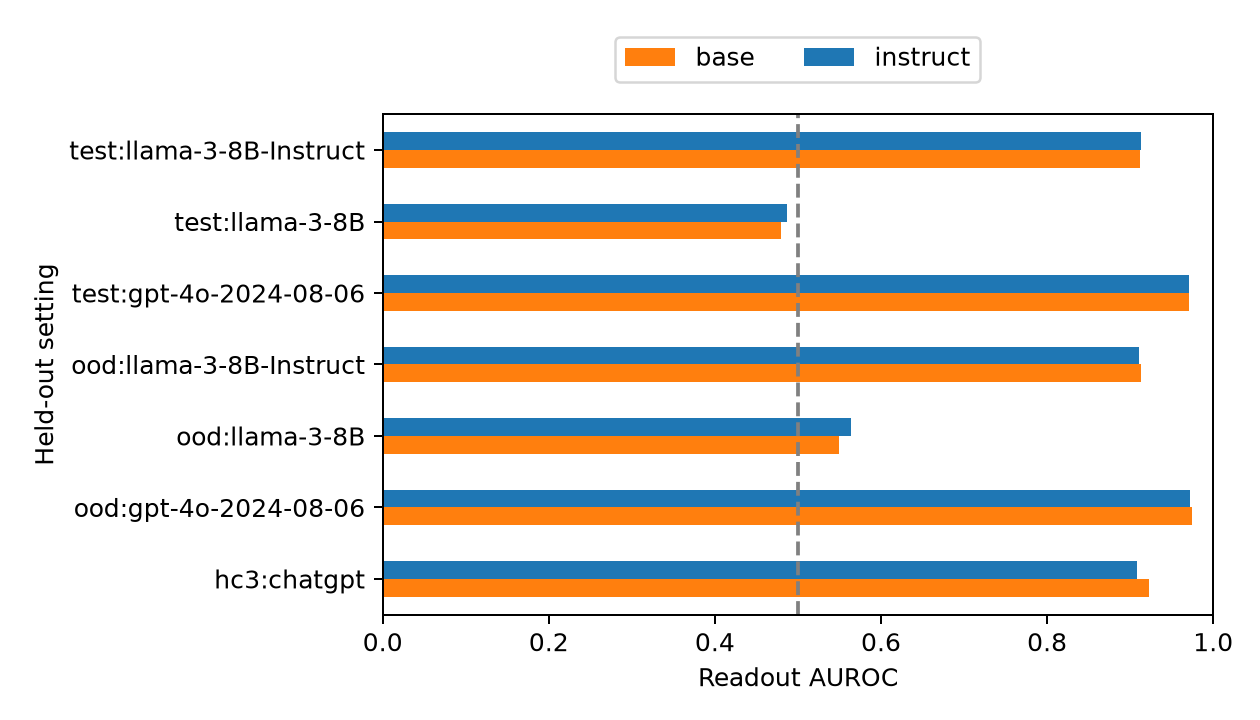
\includegraphics[width=0.95\linewidth]{figures/readout.png}
\caption{Validation-selected mean-direction readout AUROC by backbone and held-out setting. Each generator-setting uses 128 human/machine source pairs; human references are shared within each source set. The dashed line denotes chance AUROC. The plot shows point estimates; intervals and logistic alternatives are cached with the readout results. Transfer to Llama base is much weaker than transfer to instruction-generated text.}\label{fig:readout}
\end{figure}

\subsection{Observed failures}
The instruction baseline already has mean unsupported-claim fraction 0.179, and only 14.8\% of its outputs meet the requested 70--100-word range. Under mean $-2$, the proportion rated below coherence 4 rises from 5.5\% to 21.9\%. Under mean $+2$, detected Chinese/Cyrillic-script mixing occurs in 3.9\% of outputs, versus 1.6\% at zero, and truncation occurs in 2.3\%. These are descriptive flags, not grounds for removing outputs.

In the fixed first-library-task comparison recorded in the report, zero invents an anniversary; mean $-2$ invents an end time and duration and calls ``13:00'' noon; mean $+2$ adds ornate promotion and a Chinese ending. The example was fixed by prompt order rather than selected for favorable steering. Other observed failures include invented target audiences or refreshments, omitted registration deadlines, exaggerated claims, and awkward quantity descriptions. Full paired text and lowest-rated outputs are preserved in \path{results/paired_examples.json} and \path{results/failure_examples.json}. These errors explain why source-fact coverage alone is inadequate: an output can retain supplied facts while adding false claims.
